\section{Functional Requirements}
\subsection{Introduction}

\subsubsection{Scope}
The Yoco utility should be implemented within the current AutoMart system and should not replace it. The subsystem needs to provide features that will help AutoMart reduce the number of poor and irrelevant advertisements on their website.

In this regard, the utility acts as a firewall that blocks bad quality images from entering the database while also validating that images that do pass as good quality, are well represented in the advertisement.

The first test checks if the image uploaded contains a car. If the system detects a car in the image, the test is seen as successful and goes on to the next test. If the system does not detect a car in the image, further image tests come to a halt and the user is notified that a car could not be detected in the image. The system proceeds onto the next image that the user uploaded (if any).
The second test determines the colour of the car. AutoMart currently has sixteen colour buckets that the user can select from when entering the colour of the car. The system needs to calculate which colour bucket is the closest to the car's colour. The three most dominant colour buckets are then stored in the image bucket (since we need to take into account shading, lighting and other variations of colour shades on the car). Further testing can proceed even if the system was unable to determine the colour. 
The third test tries to determine the make of the car. The system uses textual data to help it determine the make, as determining the make blindly will be too time consuming. The detected make is stored in the image object and proceeds onto the final test. If the system was unable to detect a make of the car, the testing comes to a halt. 
The fourth test is the image quality test where factors such as coverage (i.e. how much of the image is actually of the car) and resolution (making use of a blur detection algortihm) are considered. These factors will help determine the rating of the image and ultimately whether the image is of sufficient quality or not.

A viable option to make sure that the car detection does not get called for a poor quality image, an additional blur detection stage could be performed as the first stage with a lenient threshold for passing the test.

After all the images have been put through the above tests, the image objects representing the images are  put through a final set of tests to ensure that there is no information conflict. The system first checks if all the objects have the same colour. If the colour differs between the objects, the system will conclude that the images represent different cars. This would mean that the advertisement is invalid, and the advert will not be allowed to be uploaded to the system until all conflicts are resolved. The second test compares all the make information. If a conflict is encountered the same principles as hold as with colour conflicts. Finally, the last test compares all the model information. The model testing will be more lenient than the first two tests. If the models differ in most of the objects and also differ from textual data, the textual data will be used to state the model of the car. 

The user will have to resolve any of the contradictions or exceptions the utility may raise before being able to submit the advertisement.
\pagebreak
\begin{figure}[h!]
  \caption{High Level System Use Case Diagram.}
  \centering
	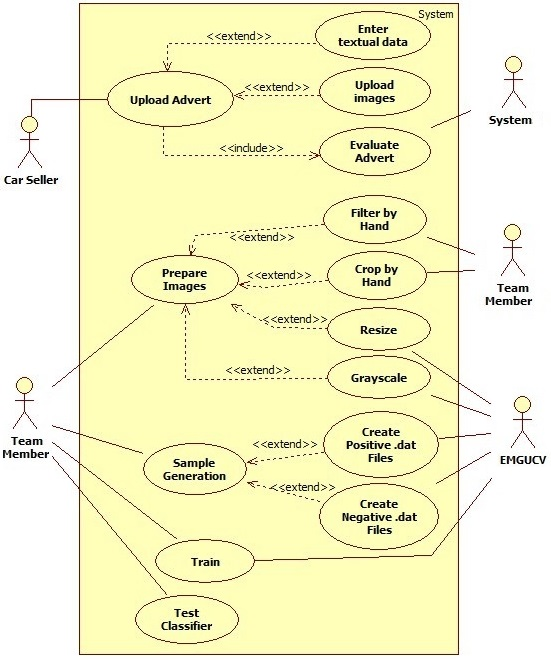
\includegraphics{HighLevelSystemUseCase.jpg}
\end{figure}

\subsubsection{Limitations}
The system may be limited on model recognition, as sometimes it is not possible to distinguish the model of the car by only face value properties that are given by an image. Therefore the system may not be able to determine the model of the car correctly every time.

\subsubsection{Exclusions}
The system should only be implemented to work with cars and should not cater for the existence of any other vehicles such as motorcycles and trucks.

\subsection{Required Functionality}
\begin{figure}[h!]
  \caption{Detect Car Low Level Use Case Diagram.}
  \centering
	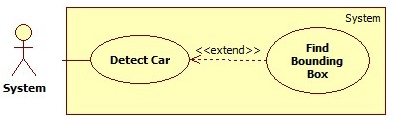
\includegraphics{DetectCarLowLevelUseCaseDiagram.jpg}
\end{figure}

\begin{figure}[h!]
  \caption{Describe Car Low Level Use Case Diagram.}
  \centering
	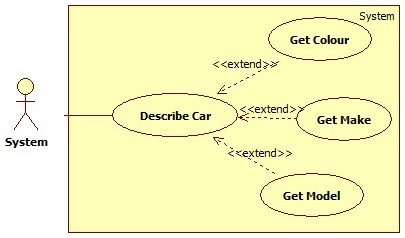
\includegraphics{DescribeCarLowLevelUseCaseDiagram.jpg}
\end{figure}

\begin{figure}[h!]
  \caption{Generate Rating Low Level Use Case Diagram.}
  \centering
	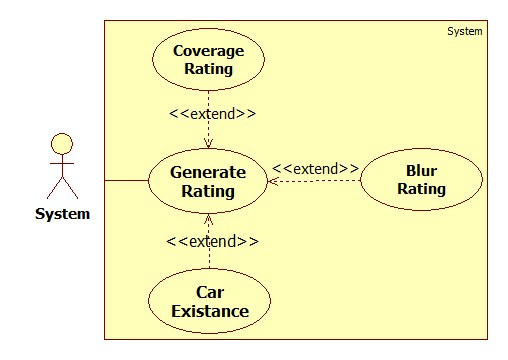
\includegraphics{GenerateRatingLowLevelUseCaseDiagram.jpg}
\end{figure}

\subsection{Use Cases}
\textbf{Detect Car Subsystem}\\
\begin{tabular}{ | l | l |}
	\hline
  	\multicolumn{2}{| c |}{\textbf{Find Bounding Box}} \\
  	\hline
  	\multicolumn{2}{| c |}{Determines if the car exists in the photo and returns co-ordinates of the box containing the car.}\\
	\hline
	Priority & Critical \\	
  	\hline
  	Pre-Conditions & A valid image needs to be provided.\\
  	\hline
 	Post-Conditions & Car detection status provided.\\
  	\hline
\end{tabular}\\
\\
\\
\textbf{Describe Car Subsystem}\\
\begin{tabular}{ | l | l | }
	\hline
  	\multicolumn{2}{| c |}{\textbf{Determine Colour}} \\
  	\hline
  	\multicolumn{2}{| c |}{Determines the colour of the car and finds the closest 3 colour buckets.}\\
	\hline
	Priority & Important \\	
  	\hline
  	Pre-Conditions & A car needs to exist in the bounding box.\\
  	\hline
 	Post-Conditions & Colour(s) of the car determined.\\
  	\hline
\end{tabular}\\
\\
\\
\begin{tabular}{ | l | l | }
	\hline
  	\multicolumn{2}{| c |}{\textbf{Determine Make}} \\
  	\hline
  	\multicolumn{2}{| c |}{Determines the make of the car.}\\
	\hline
	Priority & Nice to have \\	
  	\hline
  	Pre-Conditions & A car needs to exist in the bounding box. A make classifier needs to exist.\\
  	\hline
 	Post-Conditions & Make status determined.\\
  	\hline
\end{tabular}\\
\\
\\
\begin{tabular}{ | l | l | }
	\hline
  	\multicolumn{2}{| c |}{\textbf{Determine Model}} \\
  	\hline
  	\multicolumn{2}{| c |}{Determines the model of the car.}\\
	\hline
	Priority & Nice to have \\	
  	\hline
  	Pre-Conditions & A car needs to exist in the bounding box.\\
  	\hline
 	Post-Conditions & Model status determined.\\
  	\hline
\end{tabular}\\
\\
\\
\textbf{Generate Rating Subsystem}\\
\begin{tabular}{ | l | l | }
	\hline
  	\multicolumn{2}{| c |}{\textbf{Get Colour Value}} \\
  	\hline
  	\multicolumn{2}{| c |}{Returns a weighted value based whether the colour has been determined or not.}\\
	\hline
	Priority & Important \\	
  	\hline
  	Pre-Conditions & Use case "Determine Colour" was executed successfully.\\
  	\hline
 	Post-Conditions & Colour value successfully calculated and returned.\\
  	\hline
\end{tabular}\\
\\
\\
\begin{tabular}{ | l | l | }
	\hline
  	\multicolumn{2}{| c |}{\textbf{Get Make Value}} \\
  	\hline
  	\multicolumn{2}{| c |}{Returns a weighted value based whether the make has been determined or not.}\\
	\hline
	Priority & Important \\	
  	\hline
  	Pre-Conditions & Use case "Determine Make" was executed successfully.\\
  	\hline
 	Post-Conditions & Make value successfully calculated and returned.\\
  	\hline
\end{tabular}\\
\\
\\
\begin{tabular}{ | l | l | }
	\hline
  	\multicolumn{2}{| c |}{\textbf{Get Model Value}} \\
  	\hline
  	\multicolumn{2}{| c |}{Returns a weighted value based whether the model has been determined or not.}\\
	\hline
	Priority & Important \\	
  	\hline
  	Pre-Conditions & Use case "Determine Model" was executed successfully.\\
  	\hline
 	Post-Conditions & Model value successfully calculated and returned.\\
  	\hline
\end{tabular}\\
\\
\\
\begin{tabular}{ | l | l | }
	\hline
  	\multicolumn{2}{| c |}{\textbf{Calculate Blur}} \\
  	\hline
  	\multicolumn{2}{| c |}{Stretches the bounding box to 480x320 pixels and calculates and returns the blur value.}\\
	\hline
	Priority & Important \\	
  	\hline
  	Pre-Conditions & Bounding box exists.\\
  	\hline
 	Post-Conditions & Blur value successfully calculated and returned.\\
  	\hline
\end{tabular}\\
\\
\\
\begin{tabular}{ | l | l | }
	\hline
  	\multicolumn{2}{| c |}{\textbf{Calculate Position}} \\
  	\hline
  	\multicolumn{2}{| c |}{Determines where in the photo the car is placed, and returns the value based on the position.}\\
	\hline
	Priority & Important \\	
  	\hline
  	Pre-Conditions & Bounding box exists.\\
  	\hline
 	Post-Conditions & Car position value successfully calculated and returned.\\
  	\hline
\end{tabular}\\
\\
\\
\begin{tabular}{ | l | l | }
	\hline
  	\multicolumn{2}{| c |}{\textbf{Calculate Coverage}} \\
  	\hline
  	\multicolumn{2}{| c |}{Calculates the coverage the car occupies in the photo.}\\
	\hline
	Priority & Important \\	
  	\hline
  	Pre-Conditions & Bounding box exists.\\
  	\hline
 	Post-Conditions & Car coverage  value successfully calculated and returned.\\
  	\hline
\end{tabular}\\
\\
\\
\begin{tabular}{ | l | l | }
	\hline
  	\multicolumn{2}{| c |}{\textbf{Calculate Resolution}} \\
  	\hline
  	\multicolumn{2}{| c |}{.}\\
	\hline
	Priority & Important \\	
  	\hline
  	Pre-Conditions & Valid image provided.\\
  	\hline
 	Post-Conditions & Photo resolution value successfully calculated and returned.\\
  	\hline
\end{tabular}\\
\\
\\
\begin{tabular}{ | l | l | }
	\hline
  	\multicolumn{2}{| c |}{\textbf{Calculate Contrast}} \\
  	\hline
  	\multicolumn{2}{| c |}{Calculates contrast ratio of the photo.}\\
	\hline
	Priority & Important \\	
  	\hline
  	Pre-Conditions & Valid image provided.\\
  	\hline
 	Post-Conditions & Photo contrast value successfully calculated and returned.\\
  	\hline
\end{tabular}\\
\pagebreak
\subsection{Process Specifications}
\begin{figure}[h!]
  \caption{Activity diagram of FindBoundingBox}
  \centering
	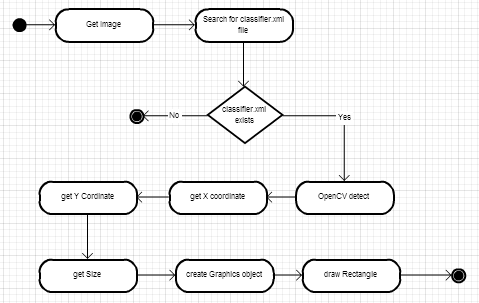
\includegraphics{activity.PNG}
\end{figure}
